
\section{Auswertung}
\label{sec:auswertung}

\subsection{Besselfunktionen}
\label{sec:bessel}

In Aufgabe 1 sollten die sphärischen Bessel-Funktionen als Funktion
von x berechnet werden und deren Nullstellen berechnet
werden. Fig.~\ref{img.bessel} zeigt die ersten 10
Bessel-Funktionen. Die Nullstellen der ersten 100 Bessel-Funktionen
befinden sich im Anhang im Unterordner ``zero-points''.

Ab der Bessel-Funktion $j_{67}$ haben die Bessel-Funktionen im
Intervall $x = 0 \ldots 100$ keine Nullstellen mehr, also insbesondere
auch $j_{125}$ nicht.

Die Wellenzahlen für $R = \unit{5}{fm}$ befinden sich ebenfalls im
Anhang im Unterordner ``wave-numbers''.

Die Orthogonalität der Besselfunktionen konnte ebenfalls gezeigt
werden, die Ergebnisse befinden sich im Anhang im Unterordner
``otho''. Es wurde dabei die Differenz zur Einheitsmatrix aufgetragen,
also $| M - 1 |$.

\begin{figure}[htbp]
  \centering
  \subfigure[]{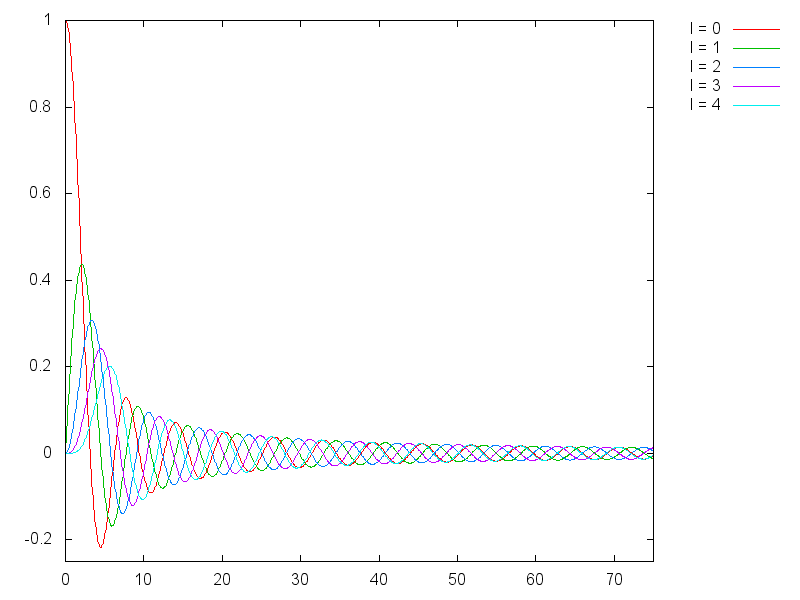
\includegraphics[width=0.45\textwidth]{img/bessel-01234}}
  \subfigure[]{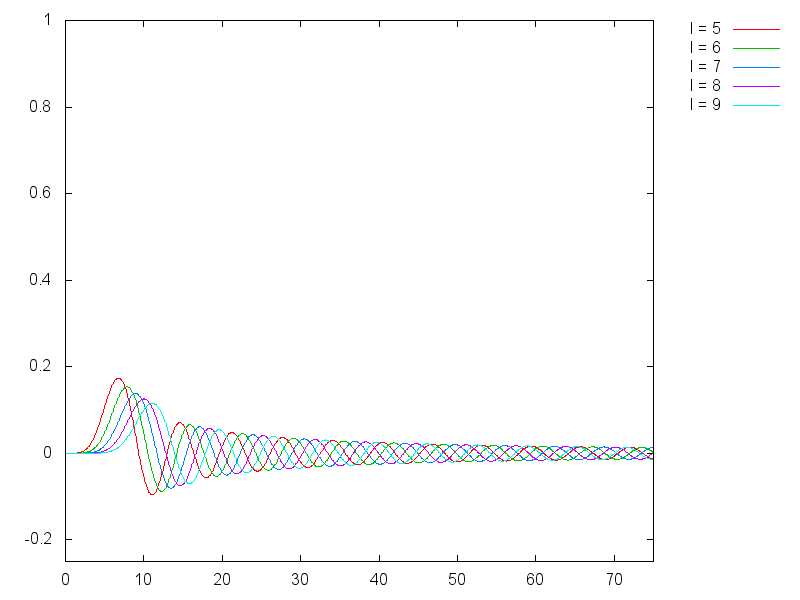
\includegraphics[width=0.45\textwidth]{img/bessel-56789}}
  \caption{Die ersten 10 sphärischen Bessel-Funktionen als Funktion von x}
  \label{img.bessel}
\end{figure}

\subsection{Diagonalisierung}
\label{sec:diag}

In Aufgabe 2 sollten die Matrizen

\begin{align}
  A_{ij} = \frac{N}{i+j} + i +j
\end{align}

für $A \in \mathbb{R}^{N \times N}$ diagonalisiert werden. Dazu wurde
das Jacobi-Verfahren verwendet. Die Ergebnisse befinden sich im Anhang
im Unterordner ``diag''.

\subsection{Schrödingergleichung eines Nukleons}
\label{sec:sgl-nukleon}

In Aufgabe 3 sollte die Bewegung eines Nukleons im
Wood-Saxon-Potential (Fig.~\ref{fig:wood-saxon}) eines Atomkerns
untersucht werden. Dazu wurden die stationären Lösungen der
Schrödingergleichung berechnet. Für eine Box-Größe $R = \unit{10}{fm}$
erhält man als Ergebnis für die Energien $E_{l,j}$:

\begin{align}
  E_{0,1} &= \unit{-40.37}{MeV} \\
  E_{0,3} &= \unit{-4.12}{MeV} \\
  E_{1,2} &= \unit{-23.47}{MeV} \\
  E_{2,2} &= \unit{-5.43}{MeV}
\end{align}

Die genauen Energie-Werte für das jeweilige $l$ befinden sich im
Anhang im Unterordner ``energy''.

Mit diesen Lösungen wurden die Wellenfunktionen

\begin{align}
  \varPsi_j(r) = \sum_i A_{ij} \cdot \alpha_{i,l} \cdot j_l(k_{i,l} \cdot r)
\end{align}

berechnet, wobei $A$ die Transformationsmatrix aus dem
Jacobi-Verfahren ist und $\alpha_{i,l}$ der Norm-Faktor zur
Besselfunktion $j_l$ und der $i$-ten Wellenzahl $k_{i,l}$. Das
Ergebnis ist in Fig.~\ref{fig:wave-functions} geplottet. Die genauen
Werte befinden sich im Anhang im Unterordner ``psi''.

\begin{figure}[htbp]
  \centering
  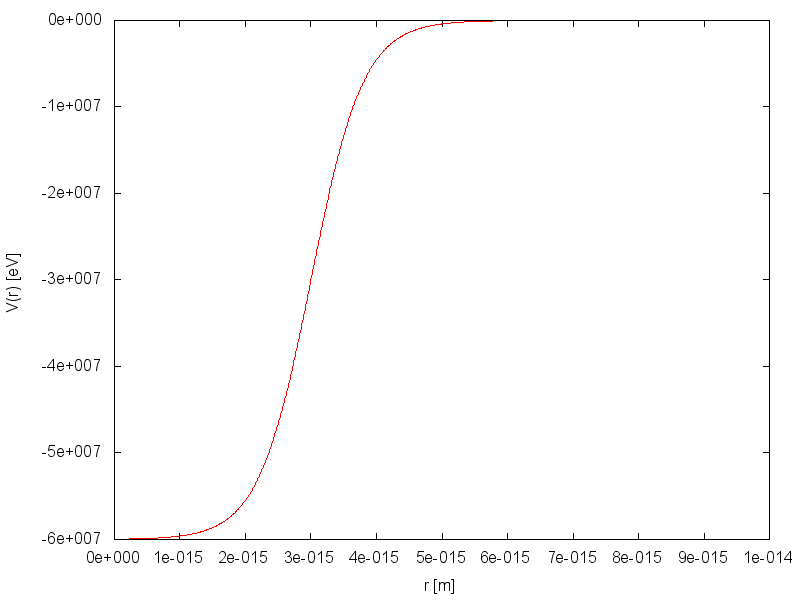
\includegraphics[width=0.9\textwidth]{img/wood-saxon}
  \caption{Das im Versuch verwendete Wood-Saxon-Potential}
  \label{fig:wood-saxon}
\end{figure}

\begin{figure}
  \centering
  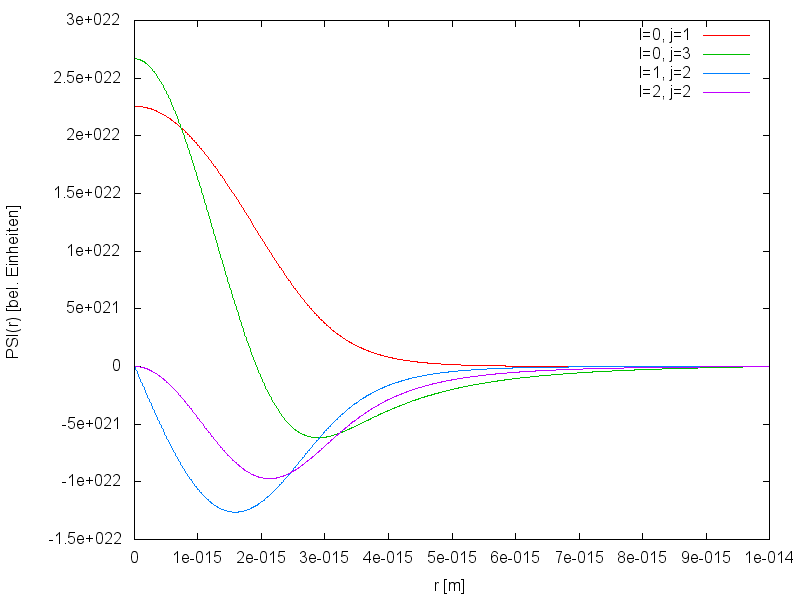
\includegraphics[width=0.9\textwidth]{img/psi}
  \caption{Wellenfunktionen $\varPsi_j(r)$ der stationären Lösungen}
  \label{fig:wave-functions}
\end{figure}

\subsection{Numerische Stabilität}
\label{sec:numerische-stabi}

Zum überprüfen der numerischen Stabilität wurde die Boxgröße und die
Zahl der Basisfunktionen angepasst. Es wurden Boxgrößen von $R =
\unit{5}{fm}, \unit{10}{fm}, \unit{15}{fm}$ gewählt und die Anzahl der
Basisfunktionen $l_{\max} = 5,10$ für jeden Wert jeweils variiert.

Für die stationären Energien $E_{l,j}$ erhält man für $R =
\unit{5}{fm}$ und $l_{\max} = 5$:

\begin{align}
  E_{0,0} &= \unit{-40.33}{MeV} \\
  E_{0,1} &= \unit{-1.22}{MeV} \\
  E_{1,0} &= \unit{-23.24}{MeV} \\
  E_{2,0} &= \unit{-4.35}{MeV}
\end{align}

Für $R = \unit{5}{fm}$ und $l_{\max} = 10$ gilt:

\begin{align}
  E_{0,0} &= \unit{-40.34}{MeV} \\
  E_{0,1} &= \unit{-1.22}{MeV} \\
  E_{1,0} &= \unit{-23.24}{MeV} \\
  E_{2,0} &= \unit{-4.35}{MeV}
\end{align}

% Für $R = \unit{10}{fm}$ und $l_{\max} = 5$ gilt:

% \begin{align}
%   E_{0,1} &= \unit{-40.37}{MeV} \\
%   E_{0,3} &= \unit{-4.12}{MeV} \\
%   E_{1,2} &= \unit{-23.47}{MeV} \\
%   E_{2,2} &= \unit{-5.43}{MeV}
% \end{align}

% Für $R = \unit{10}{fm}$ und $l_{\max} = 10$ gilt:

% \begin{align}
%   E_{0,1} &= \unit{-40.37}{MeV} \\
%   E_{0,3} &= \unit{-4.12}{MeV} \\
%   E_{1,2} &= \unit{-23.47}{MeV} \\
%   E_{2,2} &= \unit{-5.43}{MeV}
% \end{align}

Für $R = \unit{15}{fm}$ und $l_{\max} = 5$ gilt:

\begin{align}
  E_{0,2} &= \unit{-40.37}{MeV} \\
  E_{0,6} &= \unit{-4.14}{MeV} \\
  E_{1,6} &= \unit{-23.47}{MeV} \\
  E_{2,5} &= \unit{-5.43}{MeV}
\end{align}

Für $R = \unit{15}{fm}$ und $l_{\max} = 10$ gilt:

\begin{align}
  E_{0,2} &= \unit{-40.37}{MeV} \\
  E_{0,6} &= \unit{-4.14}{MeV} \\
  E_{1,6} &= \unit{-23.47}{MeV} \\
  E_{2,5} &= \unit{-5.43}{MeV}
\end{align}

Die stationären Energien $E_{j,l}$ ändern sich also nicht (nur
unwesentlich) mit höherer Ordnung der Basisfunktionen für ein festes
$R$. Auch die Werte der stationären Energien entsprechen bis auf
kleine Abweichungen für $R = \unit{5}{fm}$ bei den Energien $E_{0,1}$
und $E_{2,0}$ den Werten für $R = \unit{10}{fm}$. Für $R =
\unit{15}{fm}$ nahezu identisch. Lediglich die Ordnungen des
jeweiligen stationären Zustandes ändert sich in Abhängigkeit der
Boxgröße $R$.

Die Wellenfunktionen entsprechen im wesentlichen der Wellenfunktion
für $R = \unit{10}{fm}$ und $l_{\max} = 3$ aus Aufgabenteil 2.3.a. Die
Wellenfunktion zu $R = \unit{15}{fm}$ und $E_{2,5}$ scheint sich
jedoch invertiert zu haben.

\begin{figure}[htbp]
  \centering
  \subfigure[]{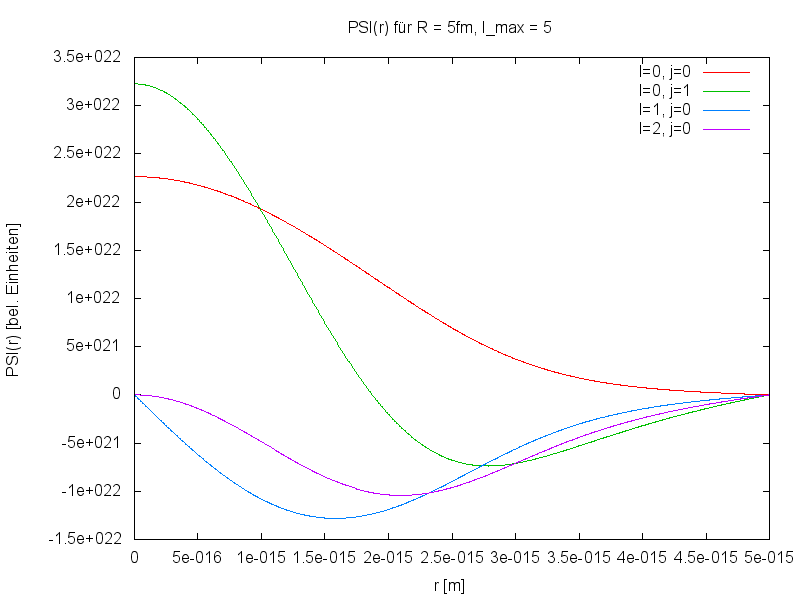
\includegraphics[width=0.45\textwidth]{img/psi-var-5-bf-5}}
  \subfigure[]{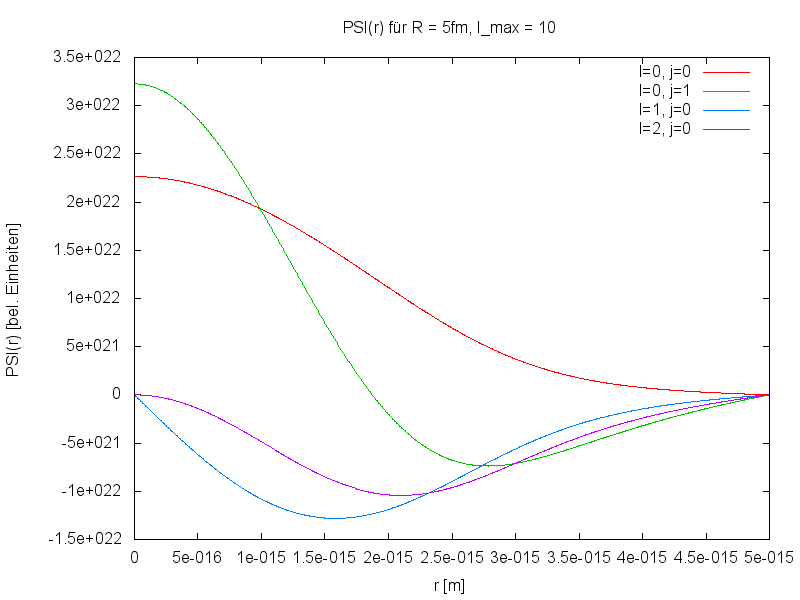
\includegraphics[width=0.45\textwidth]{img/psi-var-5-bf-10}}
  \caption{Wellenfunktion $\psi_j(r)$ für $R = \unit{5}{fm}$ und
    $l_{\max} = 5$ (links) bzw. $l_{\max} = 10$ (rechts)}
  \label{img.psi-var-5}
\end{figure}

\begin{figure}[htbp]
  \centering
  \subfigure[]{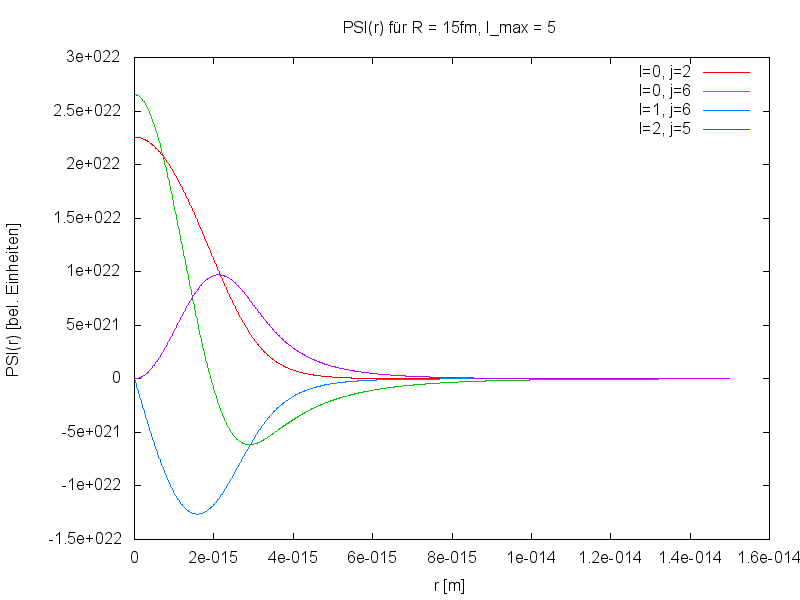
\includegraphics[width=0.45\textwidth]{img/psi-var-15-bf-5}}
  \subfigure[]{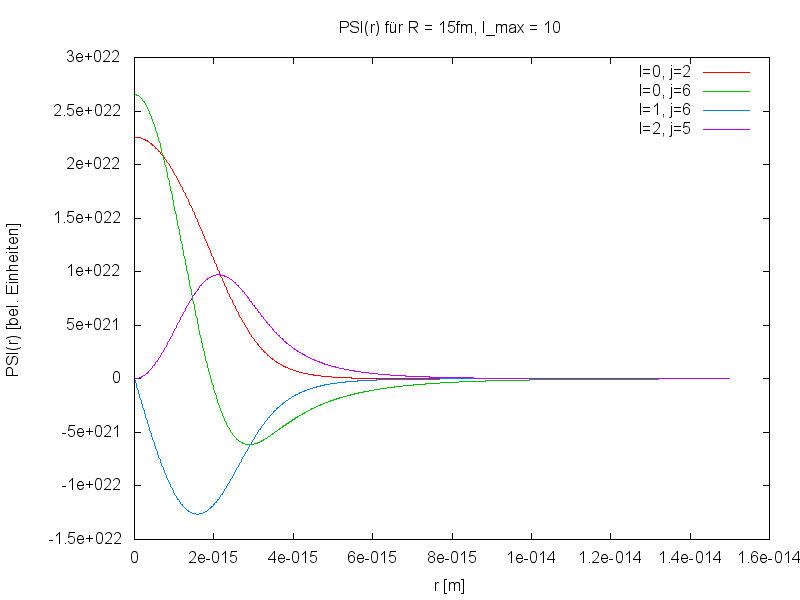
\includegraphics[width=0.45\textwidth]{img/psi-var-15-bf-10}}
  \caption{Wellenfunktion $\psi_j(r)$ für $R = \unit{15}{fm}$ und
    $l_{\max} = 5$ (links) bzw. $l_{\max} = 10$ (rechts)}
  \label{img.psi-var-5}
\end{figure}

%%% Local Variables: 
%%% mode: latex
%%% TeX-master: "protokoll"
%%% End: 
